
\section{Issues and motivations (bis)}

Causal broadcast is a communication primitive that allows a process to send
messages to all processes of its distributed system (\REF). Message deliveries
follow the happen before relationship (\REF). If the sending of a message $m$
precedes the sending of a message $m'$ then all processes that deliver these two
messages need to deliver $m$ before $m'$. Otherwise they deliver them in any
order. Each process may receive a message multiple times but it delivers it
exactly once.


\begin{figure*}
  \begin{center}
    \subfloat[Part A][\label{fig:spaceproblemA}Process~B broadcasts $b$ along
    with control information $\langle B,\,1 \rangle$.]
    {\input{input/figspaceproblemA.tex}}
    \hspace{10pt}
    \subfloat[Part B][\label{fig:spaceproblemB}Process~A receives, saves in its
    local vector, delivers and forwards
    $b$. Process~B wants to add Process~C in its direct neighbors for
    causal broadcast. It sends a control message $\pi$ to Process~C using 
    Process~A as mediator.]
    {\input{input/figspaceproblemB.tex}}    
    \hspace{10pt}
    \subfloat[Part C][\label{fig:spaceproblemC}Process~A broadcasts $a$ along with
    control information $\langle A,\, 1 \rangle$. Then, it routes $\pi$ towards
    Process~C. Process~B receives $b$ but discards it, for it is already
    registered in Process~B's local vector.]
    {\input{input/figspaceproblemC.tex}}
    \hspace{10pt}
    \subfloat[Part D][\label{fig:spaceproblemD}Process~B and Process~C receive,
    save in their local vector, deliver and forward $a$. In addition, Process~B
    buffers $a$ to send it later to Process~C.]
    {\input{input/figspaceproblemD.tex}}
    \hspace{10pt}
    \subfloat[Part E][\label{fig:spaceproblemE}Process~C receives $\pi$ and 
    replies $\rho$ to Process~B.]
    {
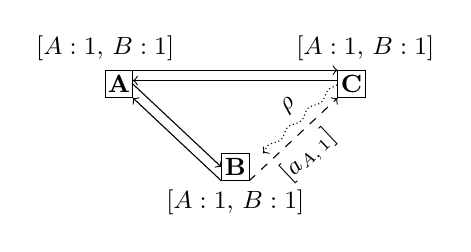
\begin{tikzpicture}[scale=1]
  
  \small
  
  \newcommand\X{210/5pt};
  \newcommand\Y{30pt};

  
  \draw[fill=white] (0*\X, 0*\Y) node{\textbf{A}} +(-5pt, -5pt) rectangle +(5pt, 5pt);
  \draw (-5+0*\X, 5+0*\Y) node[above]{$[A:1,\,B:1]$};
  \draw[fill=white] (1*\X, -1*\Y) node{\textbf{B}} +(-5pt, -5pt) rectangle +(5pt, 5pt);
  \draw (1*\X, -5-1*\Y) node[below]{$[A:1,\,B:1]$};
  \draw[fill=white] (2*\X,  0*\Y) node{\textbf{C}} +(-5pt, -5pt) rectangle +(5pt, 5pt);
  \draw (5+2*\X, 5+0*\Y) node[above]{$[A:1,\,B:1]$};
  
  \draw[->](5+0*\X, 0*\Y) -- 
  (-5+1*\X, -1*\Y); %% A->B

  \draw[<-](5+0*\X, -5+0*\Y) --
  (-5+1*\X, -5-1*\Y); %% A<-B
  
  \draw[->](5+0*\X, 5+0*\Y) --
  (-5+2*\X, 5+0*\Y); % A->C
  
  \draw[<-](5+0*\X,  1.25+ 0*\Y) --
  (-5+2*\X,  1.25+ 0*\Y); % A<-C
  
  % \draw[->,dashed](5+1*\X, -1*\Y) -- (-5+2*\X, 0*\Y); %% B<-C
 \draw[<-,densely dotted,decorate, decoration={snake, amplitude=0.3mm}](5+5+1*\X, 5+-1*\Y) -- 
 node[above, sloped]{$\bm{\rho}$}
 (-5+2*\X, 0*\Y);

  \draw[->, dashed](5+1*\X, -5-1*\Y) --
  node[sloped, below]{$[a_{A,\,1}]$} (-5+2*\X, -5+0*\Y); %% B->C



\end{tikzpicture}}
    \hspace{10pt}
    \subfloat[Part F][\label{fig:spaceproblemF}Process~B empties its buffer to
    Process~C. The latter will discard the message $a$, for it is already registered
    in Process~C's local vector]
    {\input{input/figspaceproblemF.tex}}

  \end{center}
\end{figure*}

%%% Local Variables:
%%% mode: latex
%%% TeX-master: "../paper"
%%% End:
